\chapter{图表,伪代码,公式相关排版}\label{elements}

\section{图的排版}
论文没图谁爱看呀!且看咱导言区不是已经加了``\\graphicspath{{figures/}}''吗?没错,
你要做的就是把你的图放到``figures''文件夹下面。

\subsection{单图}
单图排版很简单。

\begin{figure}[!htb]
\centering
\begin{minipage}[t]{\oneimage}
\centering
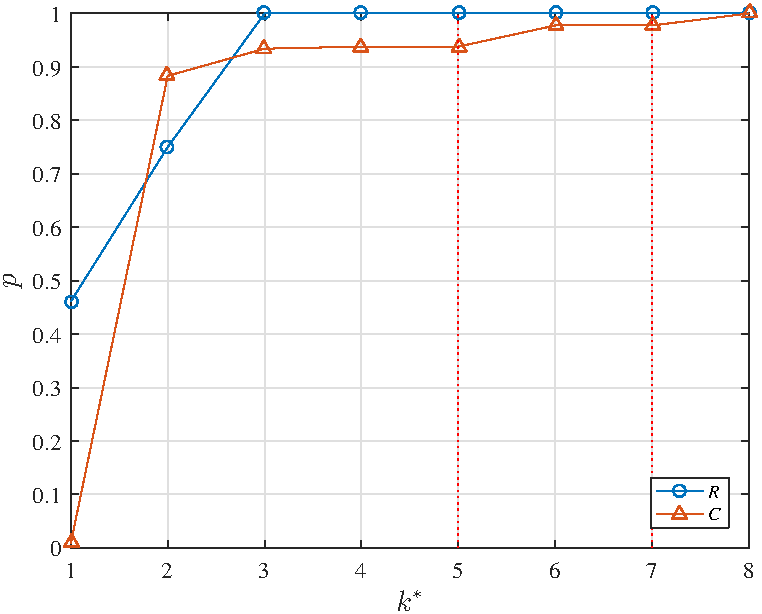
\includegraphics[width=\oneimage]{Correct_Ratio}
\end{minipage}
\caption{The ratios between the sizes of $\bm{R}$, $\bm{C}$ and their maximal possible sizes during the attack with three pairs of plain-images,
where $k^*$ denotes the index of the attacking steps.}
\label{fig:ratio}
\end{figure}

\subsection{多图}
多图排版很简单。

\begin{figure}[!htb]
\centering
\begin{minipage}[t]{\twoimage}
\centering
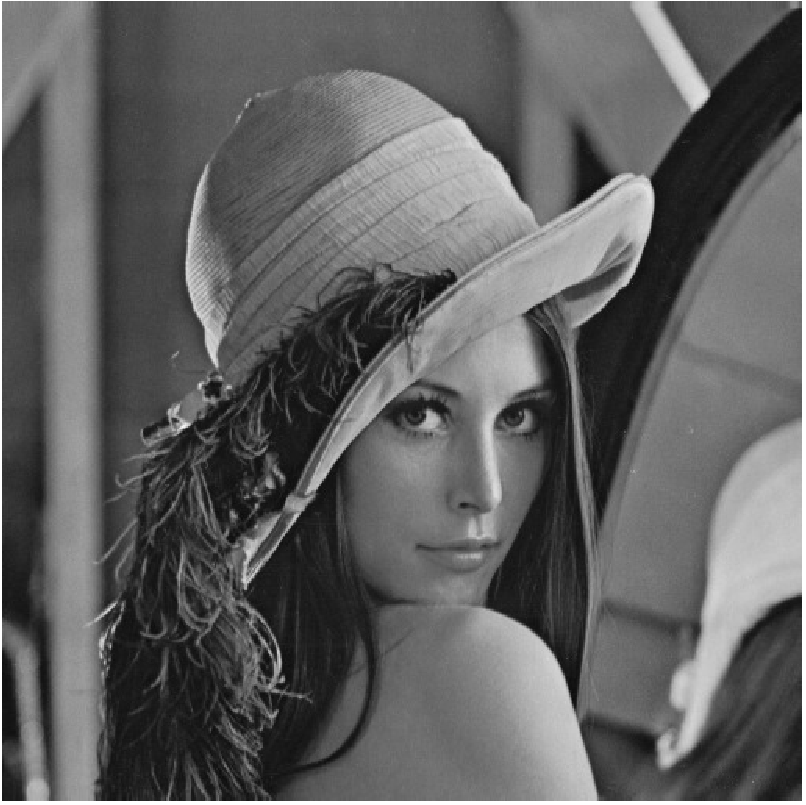
\includegraphics[width=\twoimage]{Lenna}
a)
\end{minipage} \hspace{4pt}
\begin{minipage}[t]{\twoimage}
\centering

\includegraphics[width=\twoimage]{Lenna_e}
b)
\end{minipage}
\caption{A pair of plain-image and the corresponding cipher-image:
a) image ``Lenna''; b) cipher-image of a).}
\label{fig:APairPlaintext}
\end{figure}

\section{表格}
看个例子就好了。

\begin{table}[!htb]
\centering
\caption{Blocking sizes for plain-image of size $256\times 256$.}
\label{tb:blocksize}
\begin{tabular}{c|ccc}  \hline
\backslashbox{ $q_1$ }{ $q_2$ }    & 0      & 1       & 2       \\ \hline
  0 & (8,8)  & (8,16)  & (8,32)  \\
  1 & (16,8) & (16,16) & (16,32) \\
  2 & (32,8) & (32,16) & (32,32) \\ \hline
\end{tabular}
\end{table}

\section{伪代码}
伪代码排版使用的是这方面最新的包algorithm2e,我们来看看算法\ref{qsort}(更多样例请google``algorithm2e''):

\begin{algorithm}[H]\label{qsort}
    \SetAlgoLined
    \KwData{this text}
    \KwResult{how to write algorithm with \LaTeX2e }
    initialization\;
    \While{not at end of this document}{
        read current\;
        \eIf{understand}{
            go to next section\;
            current section becomes this one\;
        }{
            go back to the beginning of current section\;
        }
    }
    \caption{How to write algorithms}
\end{algorithm}

\section{公式排版}
论文没公式的话,难道你在写散文?
已知$a+b=c$,那么

\begin{equation*}\label{eq:aplusb}
  a=c-b.
\end{equation*}

来看公式\ref{eq:aplusb}:

\begin{equation}\label{eq:amultib}
  a*b=c.
\end{equation}
